\documentclass[a4paper,11pt]{article}
\usepackage[utf8]{inputenc}
\usepackage[spanish]{babel} 
\usepackage{hyphenat}
\usepackage[hidelinks]{hyperref}
\usepackage{graphicx}
\graphicspath{{images/}}
\usepackage{subcaption}
\usepackage{color} 
\usepackage{multirow} 
\usepackage{multicol} 
\usepackage[table]{xcolor}
\usepackage{hyperref} 
\usepackage[hypcap]{caption}
\usepackage{url} 
\usepackage{booktabs} 
\usepackage[nottoc,notlot,notlof]{tocbibind} 

\title{Análisis de los precios de algunos productos en Habana del Este.}
\vspace{3cm}
\author{Jennifer de la Caridad Sánchez Santana}
\vspace{2cm}
\date{Facultad de Mátematica y Computación}
\vspace{5mm}

\setlength{\textwidth}{155mm}
\setlength{\textheight}{210mm}
\oddsidemargin=-.25cm
\begin{document}

\newpage

\maketitle
\tableofcontents

\newpage

\section{Introducción}

Habana del Este es el municipio más extenso de la provincia La Habana, ubicado en la costa norte; en el cual se encuentran ocho consejos populares, de los que dado a su extensión y disponibilidad de productos, nos propusimos a recorrer dos de ellos, Alamar y Guanabo, el primero por ser su cabecera municipal y el segundo ya que es un lugar turístico por sus hermosas y cristalinas aguas de mar que tanto disfrutan sus bañistas.
\par\vspace{1pt}
Para la realización de este proyecto, fue necesario recorrer los consejos populares mencionados anteriormente , asi como extraer mediante fotos, los datos necesaria de tres productos, cerveza, cebolla y refresco, para empezar su estudio. Luego de visitar estos poblados,y de pasar por situaciones un poco incómodas para realizar estre primer paso, pues se comenzo a buscar la mejor forma de extraer la información y poder analizarla, encontrando así diversas bibliotecas de interés como matplotlib, folium, entre otra
 \footnote{\href{https://www.sevebrau.com/de-que-depende-el-alcohol-que-tiene-una-cerveza/}{https://www.sevebrau.com/de-que-depende-el-alcohol-que-tiene-una-cerveza/}}
\section{Objetivos}
Con la realización de este proyecto pretendemos analizar lo sucedido, según los datos recolectados,
con los productos en diferentes cuestiones, ya sea su precio promedio u otras que se mencionarán más adelante, asi como ejemplificar lo que estamos haciendo mediante el uso de graficos.

\section{Desarrollo}
Para el desarrollo de este trabajo seguiremos el curso de analizar cada uno de los productos por separado y posteriormente, un análisis de las ubicaciones donde se encontraban estos.
\subsection{Cerveza}
La cerveza es una bebida alcohólica, no destilada, siendo de su tipo, la más consumida del mundo, de la cual se derivan gran cantidad de variantes con una amplia gama de matrices, debido a las diferentes formas de elaboración y a los ingredientes utilizados.Mediante el desarrollo de este trabajo, estudiaremos varios aspectos de la cerveza, entre los que encontramos su precio medio,sus diversas marcas, volumen de alcohol, entre otros.
\footnote{\href{https://dle.rae.es/cerveza}{https://dle.rae.es/cerveza}}
\par\vspace{2pt}
El salario medio mensual en la Habana según el  ¨Anuario Estadístico de Cuba en 2021, capitulo 7:Empleo y Salario¨ es de 3902 pesos cubanos, siendo la canasta básica calculada de 1528 pesos según ¨Cúanto cuestan los alimentos en Cuba¨,
\url{https://precio-alimentos.eltoque.com }
, teniendo en cuenta que la cerveza es una de las bebidas alcolizadas más consumida en Cuba,y que cada mes posee aproximadamente cuatro fines de semana,¿cuántas cervezas se puede tomar un cubano por fin de semana?, si le quitamos 800 pesos de su salario promedio para gastos extras de ya sea darle un gusto más a sus hijos o que se haya extendido un  poco en la factura de electridad, bien, pues como se muestra en dos celdas hacia abajo, la respuesta a esta pregunta sería dos cervezas por fin de semana, utilizando su precio medio, ya que la media del precio de la cerveza en Habana del Este es de 180 pesos aproximadamente, teniendo su máximo en 350 pesos , y su mínimo de 120 ,lo cual podemos apreciar en el gráfico que se muestra a continuación de como varían los precios de la cerveza respecto a su frecuencia.
\par\vspace{2pt}
\begin{minipage}{0.5\textwidth}
  \begin{center}
      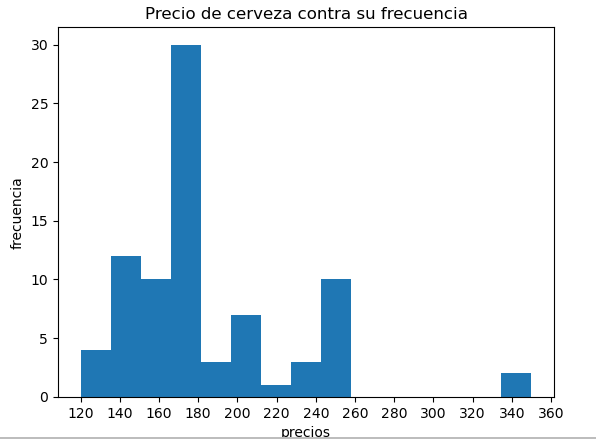
\includegraphics[width=1.3\textwidth]{precio cerveza.png}
  \end{center}
\end{minipage}
\par\vspace{2pt}
¿ Cuántos se han preguntado cuál es el volumen de alcohol promedio de la cerveza?, o han dicho, la cerveza que estoy tomando está un poco aguada(cuando tiene pocos grados), pues el por ciento de alcohol de la cerveza oscila entre los 3.5 y los 5.5 grados
\footnote{\href{https://www.sevebrau.com/de-que-depende-el-alcohol-que-tiene-una-cerveza/}{https://www.sevebrau.com/de-que-depende-el-alcohol-que-tiene-una-cerveza/}}
ya más particular, en Cuba según este estudio, oscila entre  los 4.0 y 8.6, siendo el valor medio total de 4.8 grados.
\par\vspace{2pt}
\begin{minipage}{0.5\textwidth}
  \begin{center}
      \includegraphics[width=1.3\textwidth]{volume cerveza.png}
  \end{center}
\end{minipage}
\par\vspace{2pt}
De seguro te has fijado que hay gran variedad de marcas en las cervezas que se encuentran en los diversos puntos de venta, pero sabías en Habana del Este según los datos recolectados por este estudio, habían 25 marcas diferentes, entre las que encontramos más comunes holland import y holandia premium con 10 cervezas cada una .
\par\vspace{2pt}
\begin{minipage}{0.5\textwidth}
  \begin{center}
    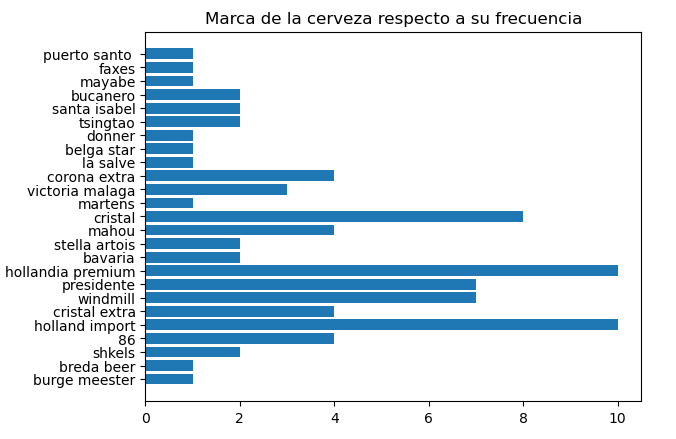
\includegraphics[width=1.8\textwidth]{marca de cerve.png}
  \end{center}
\end{minipage}
\par\vspace{2pt}
¿Cúal ustedes creen que es la marca de cerveza con mayor promedio de precio(la más cara)?, o ¿cúal es la menor?, pues la mayor es corona extra, nada más y nada menos que con un precio promedio de 250 pesos y la más barata fue puerto santo, con un promedio de 130.
\par\vspace{2pt}
\begin{minipage}{0.5\textwidth}
  \begin{center}
    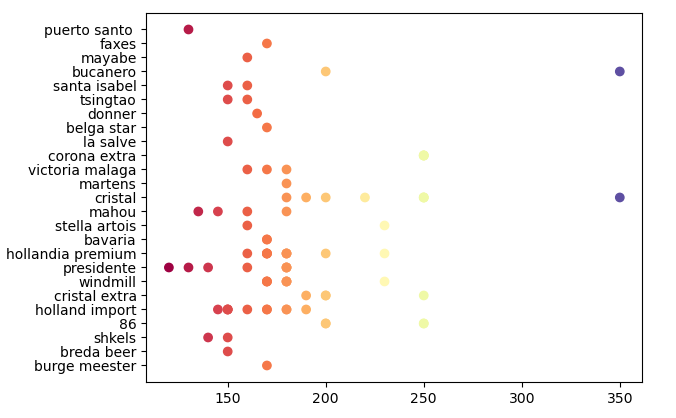
\includegraphics[width=1.7\textwidth]{marca y precio cerveza.png}
  \end{center}
\end{minipage}
\par\vspace{2pt}
Probablementre has notado que cada vez más en los diversos puntos de venta hay disminución de la cantidad  de las botellas de cerveza, ¿te has preguntado el por qué?.Ya sea por protección de la cerveza, ya que sus mayores enemigos son la luz , el calor y el oxígeno, siendo las latas fabricadas expecificamente para actuar en contra de dichos agentes, o porque es más barata su compra debido a que una lata de 355 mililitros pesa 2.2 kilos y una botella de su misma cantidad 3.4 kilos
\footnote{\href{https://www.conmuchagula.com/la-cerveza-en-lata-o-en-botella-ventajas-e-inconvenientes}{https://www.conmuchagula.com/la-cerveza-en-lata-o-en-botella-ventajas-e-inconvenientes}}
realmente en el mercado de la cerveza ha habido una notable caída de la venta en bottelas, como vemos reflejado en este estudio, donde con apenas 3 botellas nos encontramos en todo el recorrido , mientras que con latas, unas 79.
\par\vspace{2pt}
\begin{minipage}{0.5\textwidth}
  \begin{center}
    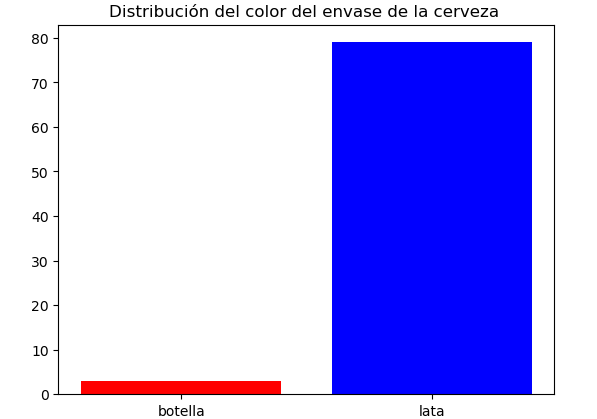
\includegraphics[width=1.7\textwidth]{envase cerveza.png}
  \end{center}
\end{minipage}
\par\vspace{2pt}
\subsection{Cebolla}
La cebolla es uno de los alimentos que no puede faltar en la cocina de nuestros hogares, ya que además de ser uno de los ingredientes base en muchas de nuestras recetas, también es rica en vitaminas y grandes beneficios para la salud.Con el desarrollo de este proyecto analizaremos datos sobre esta, así como sus variedades, precios y forma en la que se oferta.
\par\vspace{2pt}
¿Alguna vez se han puesto a pensar en si la cebolla en libras es más barata que la que se encuentra en otras categorías o viceversa?, pues sabían que la cebolla en libras(según este estudio), alcanza un precio promedio de 162 pesos aproximadamente, mientras que en el resto de las categorías, es de 318, oscilando la primera entre los 100 y los 180 pesos, mientras que el resto obtiene su mínimo en 150 y su máximo en 500, apreciando una notable diferencia, en la cual la cebolla en libras es más barata.
\par\vspace{2pt}
\begin{minipage}{0.5\textwidth}
  \begin{center}
    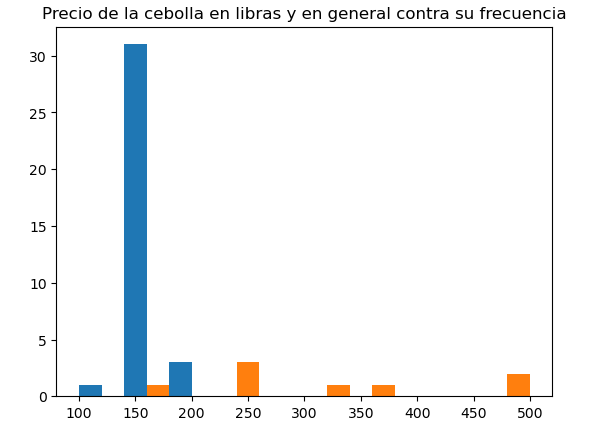
\includegraphics[width=1.5\textwidth]{precio de cebolla.png}
  \end{center}
\end{minipage}
\par\vspace{2pt}
Seguramente se han preguntado si estará pasando algo con la cebolla, por qué hay poca cebolla morada o pq la veo más cara, en verdad, la cebolla morada ha disminuido en cantidad, ya no la vemos tan comúnmente como antes en cada puesto de ventas; ¿esto habrá influido en su precio?, pues como se aprecia en el siguiente gráfico, el precio de la cebolla blanca tiene un mínimo de 100 pesos cubanos, mientras que la cebolla morada en su primera aparición posee un precio de 150 pesos, a la vez que es más común encontrar cebollas moradas en categorías que no sean libras, tiene 2 más que las blanca, casi siempre en un precio superior.
\par\vspace{2pt}
\begin{minipage}{0.5\textwidth}
\begin{center}
  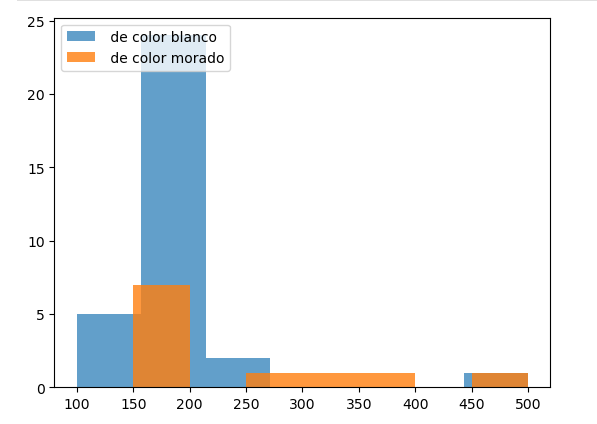
\includegraphics[width=1.5\textwidth]{precio por color cebolla.png}
\end{center}
\end{minipage}
\par\vspace{2pt}
En la realizacion de este proyecto nos topamos con 32 cebollas blancas y apenas 11 moradas, viendo como en realidad ha disminuido la oferta de cebollas moradas en Habana del Este, al menos en el tiempo de realizacon de este estudio.
\par\vspace{2pt}
\begin{minipage}{0.5\textwidth}
\begin{center}
  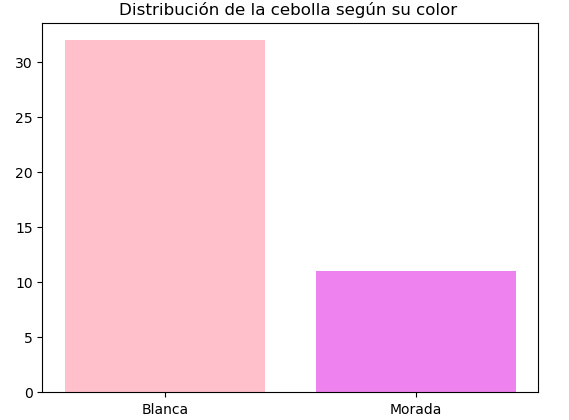
\includegraphics[width=1.5\textwidth]{color de la cebolla.png}
\end{center}
\end{minipage}
\subsection{Refresco}
Para hacer algo diferente se nos ocurrió una idea, hacer una comparación entre los refrescos embasados en botellas de plástico y en latas de aluminio para ver quien tiene más ventajas. 
1-Los refrescos en botellas de plástico:
\begin{itemize}
\item poseen acetaldehído que podrían pasar al refresco y afectar su sabor, aún en cantidades mínimas.
\item el plástico es más permeable al CO2, la efervecencia de la bebida se escapa más rápido.
\item se derivan de productos no renovables(petróleo).
\item no se puede reciclar en más botellas (si a caso en fibras de alfombras, ropas o sacos de dormir).
\item las personas no reciclan botellas de plástico tan a menudo.
\end{itemize}
\footnote{\href{https://www.elfinanciero.com.mx/food-and-drink/2022/06/14/cual-sabe-mejor-refresco-en-vidrio-plastico-0-lata/?outputType=amp}{https://www.elfinanciero.com.mx/food-and-drink/2022/06/14/cual-sabe-mejor-refresco-en-vidrio-plastico-0-lata/?outputType=amp}}
\footnote{\href{https://medialab.news-latas-de-aluminoio-vs-botellas-de-plastico-cual-afecta-mas-al-medio-ambiente/?amp}{https://medialab.news-latas-de-aluminoio-vs-botellas-de-plastico-cual-afecta-mas-al-medio-ambiente/?amp}}
2-Los refrescos en latas de aluminio:
\begin{itemize}
\item el interior de las latas está revestido con un polímero que puede contener BPA o Bishfenol A, con lo cual se evita el contacto del refresco con el metal.
\item son menos permeables al CO2, conservan las burbujas por más tiempo.
\item proviene de la roca bausita, y su extracción puede arruinar ecosistemas.
\item se pueden reciclar en nuevas latas.
\item se estima que casi el 75 porciento de aluminio producido está en uso.
\end{itemize}
Luego de haber leido los anteriores enunciados sobre ambos embaces vamos a analizar lo sucedido respecto a aspectos como el precio promedio,marca entre otros de los refrescos en latas de aluminio, gracias a que poseen ventajas sobre las botellas de pástico, sin dejar de lado que ambos tienen desventajas para el medio ambiente.
\par\vspace{2pt}
En Cuba y en especial en Habana del Este el precio del refresco en latas, posee un valor medio de 160 pesos cubanos, obteniendo un mínimo en 130, con un refresco de la marca ciego montero que nos encontramos en este recorrido, y alcanzando un valor máximo de 260 pesos, con la marca coca cola.
\par\vspace{2pt}
\begin{minipage}{0.5\textwidth}
  \begin{center}
    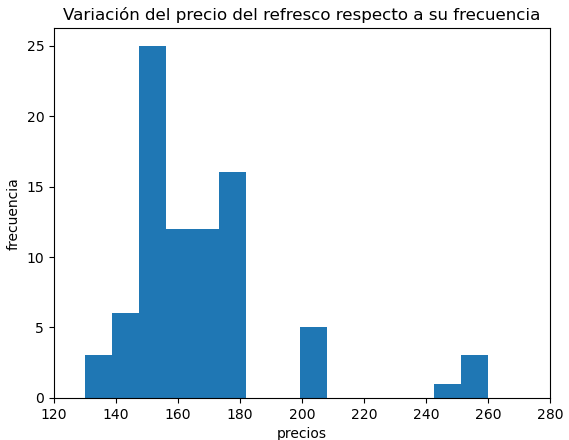
\includegraphics[width=1.4\textwidth]{precio de refresco.png}
  \end{center}
\end{minipage}
\par\vspace{2pt}
¿Cúal ustedes pensarán que es el sabor de refresco más común en nuestro días?, pues en Habana del Este según nuestros datos recolectados el refresco que más encontramos fue de sabor limón con 30 refrescos, mientras que el que menos encontré, es el de sabor piña, que como ya todos vemos en nuestros día a día es el que menos disponibilidad en los puntos de venta hay.
\par\vspace{2pt}
\begin{minipage}{0.5\textwidth}
  \begin{center}
    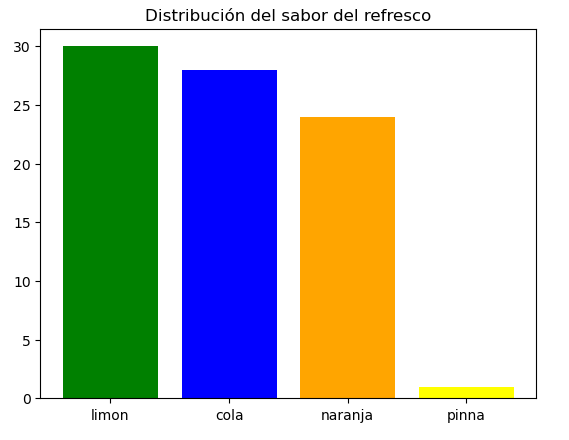
\includegraphics[width=1.4\textwidth]{sabor de refresco.png}
  \end{center}
\end{minipage}
\par\vspace{2pt}
Se han preguntado que si todavía están vendiendo refrescos cubanos de marcas como ciego montero o iron bell en las diversas cafeterías, pues la respuesta es sí, en Habana del Este incluso, los refrescos con que más nos topamos fueron de la marca ciego montero,(18), sin negar que había una gran variedad de marcas , alredor de once,  de las cuales las que menos hallamos fueron najita y cachito, con apenas un refresco de cada uno.
\par\vspace{2pt}
\begin{minipage}{0.5\textwidth}
  \begin{center}
    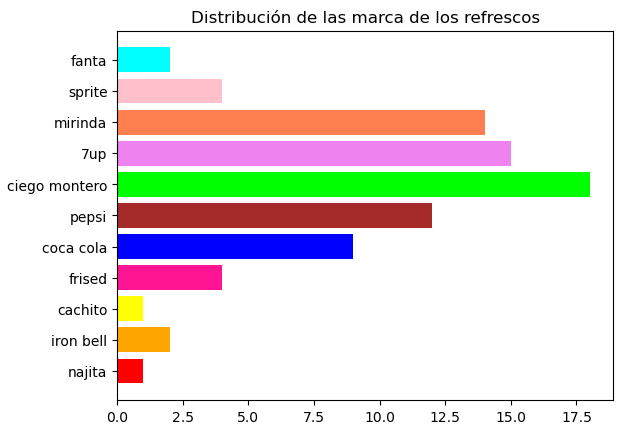
\includegraphics[width=1.4\textwidth]{marca de refresco.png}
  \end{center}
\end{minipage}
\par\vspace{2pt}
¿Cuál ustedes pensarían que es la marca con un promedio de precios más caro?, pues es tropicola, con un promedio de 200 pesos, y la más barata es frised con un promedio de 134 pesos aproximadamente.
\par\vspace{2pt}
\begin{minipage}{0.5\textwidth}
  \begin{center}
    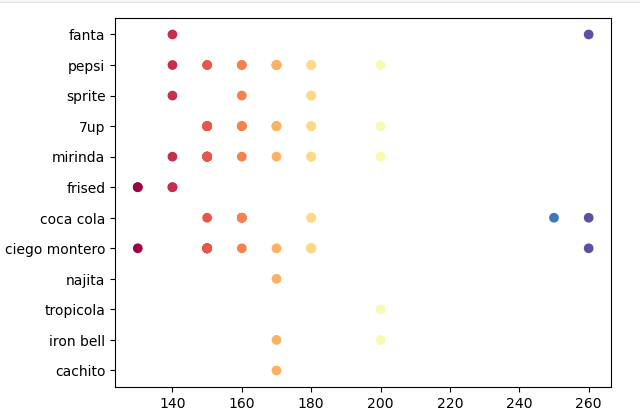
\includegraphics[width=1.4\textwidth]{marca y precio de refresco.png}
  \end{center}
\end{minipage}
\par\vspace{2pt}
Alguna vez han sentido que el día es muy caluroso, y van a una cafetería y da la casualidad que no hay cerveza, pues sabían que según los resultados de este estudio aproximadamente el 8 porciento de las cafeterías que tienen refresco no tienen cerveza, lo cual vemos reflejado en el mapa siguiente, de color rojo son los puntos que tienen refresco, y azul cerveza.
\par\vspace{2pt}
\begin{minipage}{0.5\textwidth}
  \begin{center}
    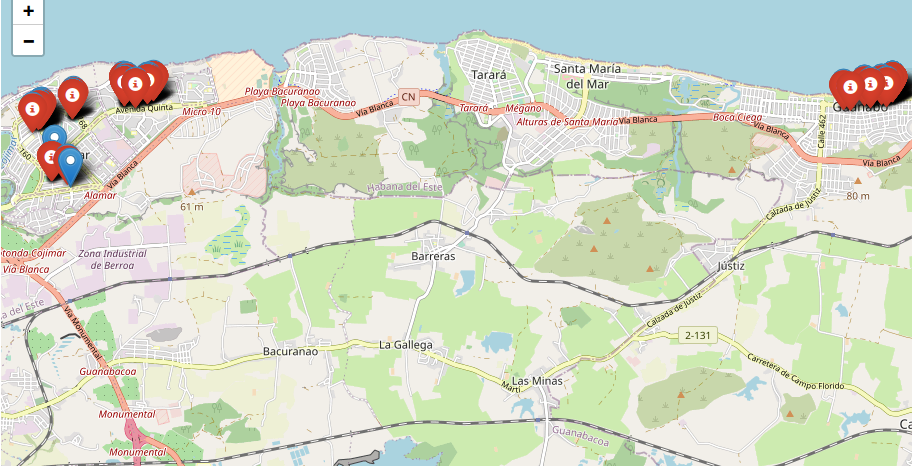
\includegraphics[width=1.4\textwidth]{mapa de cerveza y refresco.png}
  \end{center}
\end{minipage}
\par\vspace{2pt}
Muchos se preguntarán ¿cómo es la disponibilidad de cebolla en Habana del Este?, pues en ambos consejos populares que visitamos , independientemente del color de la cebolla, había gran presencia de dicho producto, como podemos apreciar en el mapa siguiente.
\par\vspace{2pt}
\begin{minipage}{0.5\textwidth}
  \begin{center}
    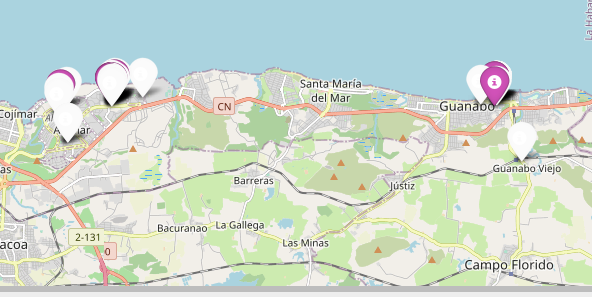
\includegraphics[width=1.4\textwidth]{mapa de cebolla.png}
  \end{center}
\end{minipage}


\newpage

\section{Conclusiones}
A modo de conclusión con la realización de este trabajo podemos enunciar lo siguiente:
\begin{enumerate}
  \item Habana del Este es un municipio bastante amplio, con grandes cantidades de puntos de ventas que ofertan a la pobloción diversos productos y una disponibilidad en dichos locales, admirable.
  \item Con la realización de este trabajo más allá de analizar algunos datos interesantes referentes a cada producto, se puedo establecer, el precio medio para la adquisición de dichos productos, teniendo la cerveza un precio promedio de 180 pesos ,de la cebolla en general, 160 y del refresco, 160 igual.  
  \item Recordamos que la extracción de nuestros datos fue realizada en los meses de abril y  mayo del año 2023, dichos datos ,se encuentran variando día a día, y pues como el mercado de los precios es algo inesacto, recomendamos, que si desea saber cuales son los precios actuales, recorra usted el municipio Habana del Este.
\end{enumerate}


\section{Referencias}
1-\url{https://www.cubatesoro.com/municipio-habana-este/}
\par\vspace{2pt}
2-\url{https://dle.rae.es/cerveza}{https://dle.rae.es/cerveza}
\par\vspace{2pt}
3-\url{https://precio-alimentos.eltoque.com}
\par\vspace{2pt}
4-\url{https://www.sevebrau.com/de-que-depende-el-alcohol-que-tiene-una-cerveza/}
\par\vspace{2pt}
5-\url{https://www.conmuchagula.com/la-cerveza-en-lata-o-en-botella-ventajas-e-inconvenientes}
\par\vspace{2pt}
6-\url{https://www.elfinanciero.com.mx/food-and-drink/2022/06/14/cual-sabe-mejor-refresco-en-vidrio-plastico-0-lata/?outputType=amp}
\par\vspace{2pt}
7-\url{https://www.medialab.news-latas-de-aluminoio-vs-botellas-de-plastico-cual-afecta-mas-al-medio-ambienteS}


\end{document}
